\documentclass[activite]{thedocument}
\usepackage{tkz-euclide}
\startdatakeys
\source{}
\cycle{}
\competencesDuSocle{}
\connaissancesRequises{}
\competencesTravaillees{}
\enddatakeys
\begin{document}
    Dans chaque cas, écrire l'expression numérique donnant $AB$.\vskip20pt
    \begin{enumerate}
        \item\hskip30pt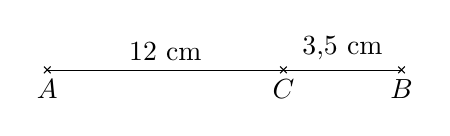
\begin{tikzpicture}[scale=1.5]
            \tkzDefPoint(0,0){A}
            \tkzDefPoint(3,0){B}
            \tkzDefPoint(2,0){C}
            \tkzDrawPoints[cross out](A,B,C)
            \tkzLabelPoints(A,B,C)
            \tkzDrawSegment(A,B)
            \tkzDefMidPoint(A,C)
            \tkzGetPoint{M}
            \tkzDefMidPoint(C,B)
            \tkzGetPoint{N}
            \draw node[above] at(M){12 cm};
            \draw node[above] at(N){3,5 cm};
        \end{tikzpicture}\vskip30pt
        \item\hskip30pt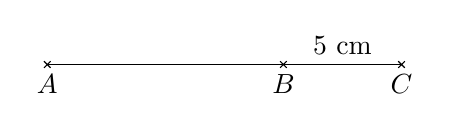
\begin{tikzpicture}[scale=1.5]
            \tkzDefPoint(0,0){A}
            \tkzDefPoint(3,0){C}
            \tkzDefPoint(2,0){B}
            \tkzDrawPoints[cross out](A,B,C)
            \tkzLabelPoints(A,B,C)
            \tkzDrawSegment(A,C)
            \tkzDefMidPoint(A,C)
            \tkzGetPoint{M}
            \tkzDefMidPoint(C,B)
            \tkzGetPoint{N}
            \draw node[above] at(N){5 cm};
        \end{tikzpicture}\par\hskip30pt$AC=21$ cm\vskip30pt
        \item\hskip30pt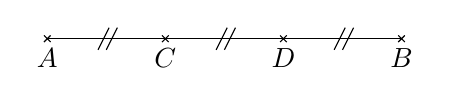
\begin{tikzpicture}[scale=1.5]
            \tkzDefPoint(0,0){A}
            \tkzDefPoint(3,0){B}
            \tkzDefPoint(1,0){C}
            \tkzDefPoint(2,0){D}
            \tkzDrawPoints[cross out](A,B,C,D)
            \tkzLabelPoints(A,B,C,D)
            \tkzDrawSegment(A,B)
            \tkzDefMidPoint(A,C)
            \tkzGetPoint{M}
            \tkzDefMidPoint(C,B)
            \tkzGetPoint{N}
            \tkzMarkSegments[mark=s||](A,C C,D D,B)
        \end{tikzpicture}\par\hskip30pt$AC=2,5$ cm
    \end{enumerate}\vskip50pt
\end{document}